\thispagestyle{cackithitoannone}
\pagestyle{cackithitoan}
\everymath{\color{cackithi}}
\graphicspath{{../cackithi/pic/}}
\blfootnote{\color{cackithi}$^1$Trường Phổ thông Năng khiếu, ĐHQG TpHCM.}
\begingroup
\AddToShipoutPicture*{\put(0,616){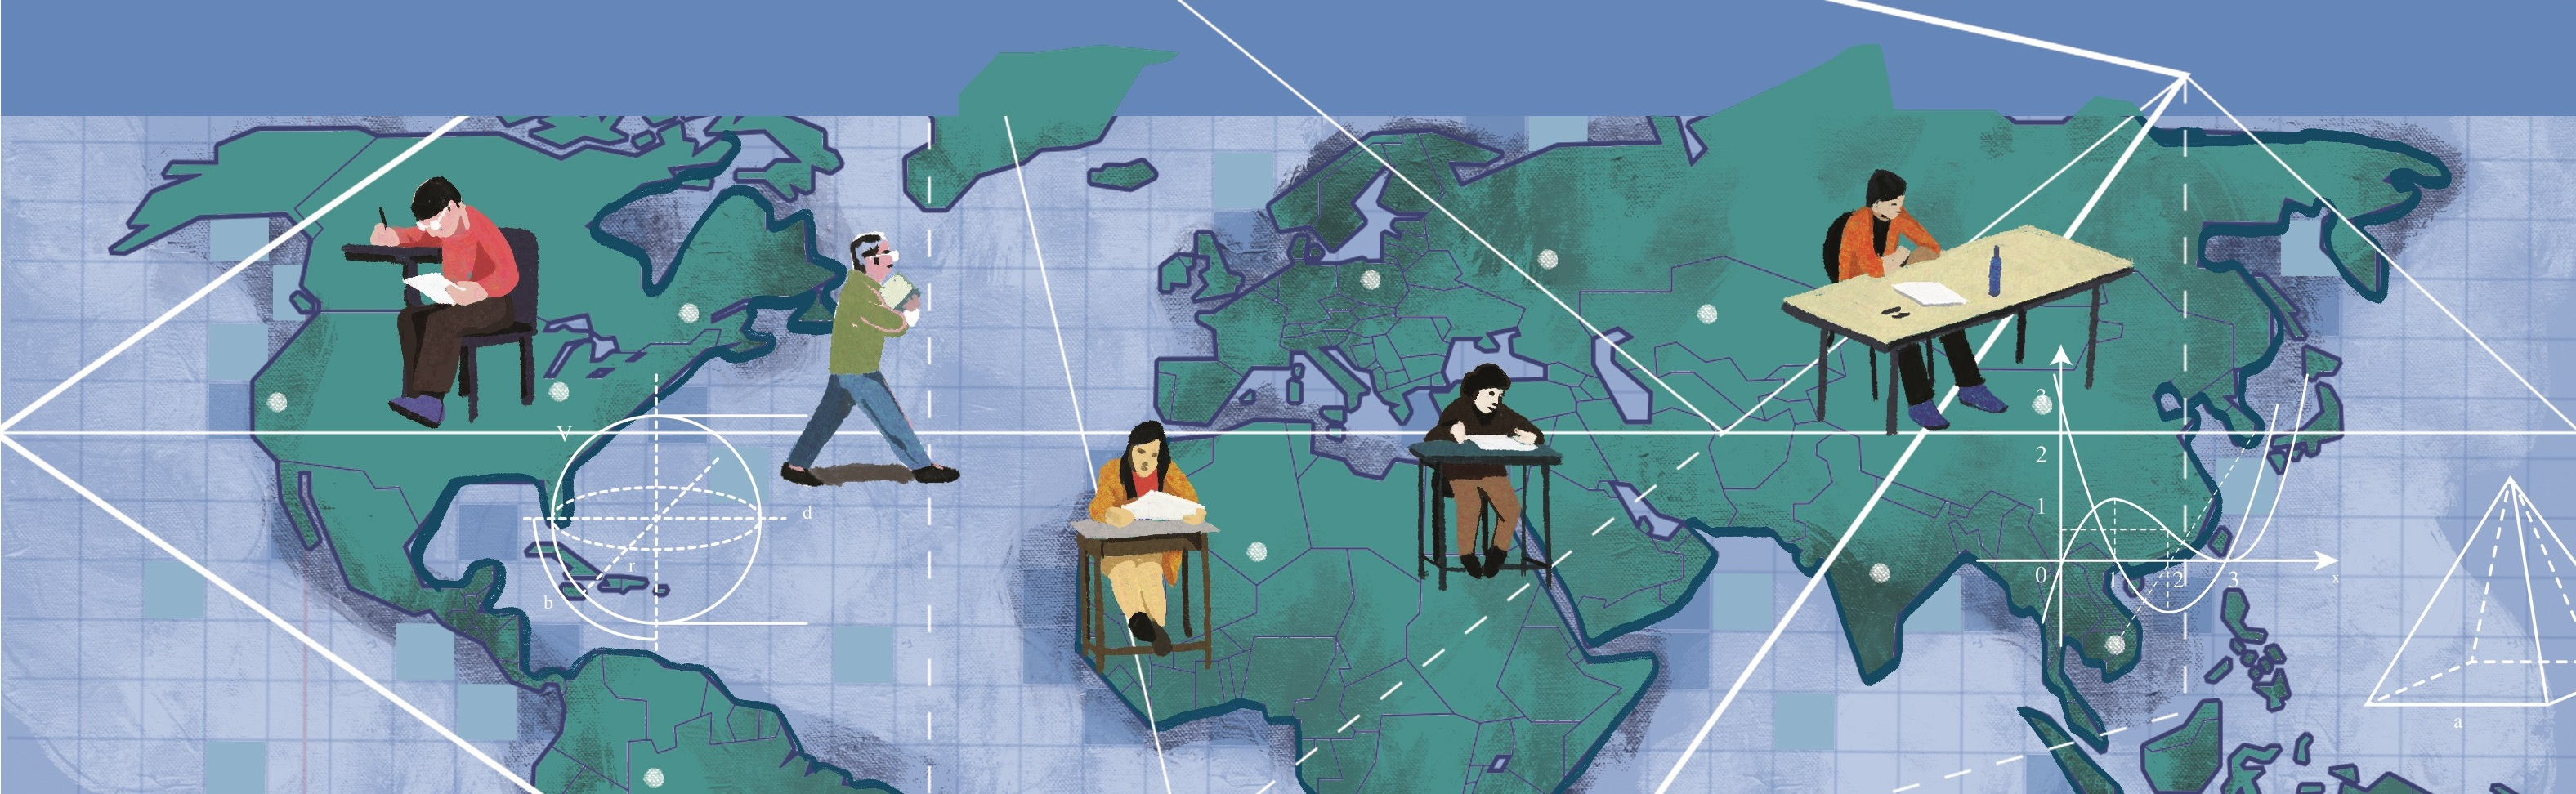
\includegraphics[width=19.3cm]{../bannercackithi}}}
\AddToShipoutPicture*{\put(52,522){
\includegraphics[scale=1]{../tieude3.pdf}}}
\centering
\endgroup
\vspace*{190pt}

\begin{multicols}{2}
	Kỳ thi chọn học sinh giỏi quốc gia năm học $2023-2024$ đã diễn ra trong hai ngày $5, 6/1/2024$. Bài viết giới thiệu đề thi môn Toán của kỳ thi năm nay cùng một số bình luận và nhận định của tác giả bài viết về đề thi này.
	\vskip 0.1cm
	Đề thi năm nay có ưu điểm là đặt các vấn đề thú vị, không theo lối mòn, đặc biệt là không đi theo một mô--típ cũ suốt hơn mười năm nay là đề thi lúc nào cũng có hai bài hình. Điều này sẽ giúp cho việc dạy và học đều hơn, hướng đến cơ bản hơn, tránh bắt tủ. Tuy vậy, đề thi cũng có những nhược điểm về cấu trúc, diễn đạt và sắp xếp làm giảm đi đáng kể những điểm tích cực. Trước khi đi đến những đánh giá chung, chúng ta đi chi tiết vào từng bài toán thi.
	\vskip 0.1cm
	\textbf{\color{cackithi}Đề bài $\pmb1$:} Với mỗi số thực $x$, ta gọi $[x]$ là số nguyên lớn nhất không vượt quá $x$.
	\vskip 0.1cm
	Cho dãy số $\{a_n\}_{n=1}^\infty$ xác định bởi: $a_n = \dfrac{1}{4^{[-\log_4 n]}}, \forall n \ge 1$. Đặt $b_n =  \dfrac{1}{n^2}\left( {\sum\limits_{k = 1}^n {{a_k}}  - \frac{1}{{{a_1} + {a_2}}}} \right), \forall n \ge 1$. 
	\vskip 0.1cm
	$a)$ Tìm một đa thức $P(x)$ với hệ số thực sao cho $b_n = P\left(\dfrac{a_n}{n}\right), \forall n \ge 1$.
	\vskip 0.1cm
	\columnbreak
	$b)$ Chứng minh rằng tồn tại một dãy số nguyên dương $\{n_k\}_{k=1}^\infty$ tăng thực sự sao cho
	\begin{align*}
		\mathop {\lim }\limits_{k \to \infty } {b_{{n_k}}} = \frac{{2024}}{{2025}}. 
	\end{align*}
	Bài toán này có định dạng khá lạ so với các bài toán dãy số trong các kỳ thi năm trước, một dãy số dưới dạng tổng đòi hỏi phần xử lý đại số trước. Mặc dù đã có hướng dẫn trước để đi đến công thức mấu chốt
	\begin{align*}
		b_n = - \dfrac{1}{5}\left(\dfrac{a_n}{n}\right)^2 + \dfrac{a_n}{n}
	\end{align*}
	nhưng đây vẫn là một ý không hề hiển nhiên. Ý thứ hai thì không khó đối với một học sinh (hoặc sinh viên) được học bài bản về giới hạn và về tập số thực, nhưng với các em học sinh chỉ vừa làm quen với giải tích thì quả là quá tầm. 
	\vskip 0.1cm
	\textbf{\color{cackithi}Đề bài $\pmb2$:} Tìm tất cả các đa thức $P(x), Q(x)$ với hệ số thực sao cho với mỗi số thực $a$ thì $P(a)$ là nghiệm của phương trình: $x^{2023} + Q(a)\cdot x^2 + (a^{2024} + a)x + a^3 + 2025a = 0$.
	\vskip 0.1cm
	Đây là một bài phương trình hàm đa thức nhẹ nhàng, chủ yếu dựa vào sự chia hết, đồng dư đa thức.
	\vskip 0.1cm
	\textbf{\color{cackithi}Đề bài $\pmb3$:} Cho $ABC$ là tam giác nhọn với tâm đường tròn ngoại tiếp $O$. Gọi $A'$ là tâm của đường tròn đi qua $C$ và tiếp xúc $AB$ tại $A$, gọi $B'$ là tâm của đường tròn đi qua $A$ và tiếp xúc $BC$ tại $B$, gọi $C'$ là tâm đường tròn đi qua $B$ và tiếp xúc $CA$ tại $C$.
	\vskip 0.1cm
	$a)$ Chứng minh rằng diện tích tam giác $A'B'C'$ lớn hơn hoặc bằng diện tích tam giác $ABC$.
	\vskip 0.1cm
	$b)$ Gọi $X,Y,Z$ lần lượt là hình chiếu vuông góc của $O$ lên các đường thẳng $A'B',B'C', C'A'$. Biết rằng đường tròn ngoại tiếp tam giác $XYZ$ lần lượt cắt lại các đường thẳng $A'B', B'C', C'A'$ tại các điểm $X',Y',Z' (X' \ne X, Y' \ne Y, Z' \ne Z)$. Chứng minh rằng các đường thẳng $AX', BY', CZ'$ đồng quy.
	\vskip 0.1cm
	Bài toán hình học này khai thác một cấu hình khá thú vị, lời giải chủ yếu sử dụng phép biến đổi góc, tam giác đồng dạng. Bài này có hai ý khá độc lập nhưng đều có thể sử dụng chung phép đồng dạng (vị tự quay) biến $ABC$ thành $A'B'C'$. Đây là năm thứ hai xuất hiện bất đẳng thức hình học và nội dung này vẫn tiếp tục gây khó khăn cho các thí sinh. 
	\vskip 0.1cm
	\textbf{\color{cackithi}Đề bài $\pmb4$:} Người ta xếp $k$ viên bi vào các ô của một bảng $2024 \times 2024$ ô vuông sao cho hai điều kiện sau được thỏa mãn: mỗi ô không có quá một viên bi và không có hai viên bi nào được xếp ở hai ô kề nhau (hai ô được gọi là kề nhau nếu chúng có chung một cạnh).
	\vskip 0.1cm
	$a)$ Cho $k = 2024$. Hãy chỉ ra một cách xếp thỏa mãn cả hai điều kiện trên mà khi chuyển bất kỳ viên bi đã được xếp nào sang một ô tùy ý kề với nó thì cách xếp mới không còn thỏa mãn cả hai điều kiện nêu trên.
	\vskip 0.1cm
	$b)$ Tìm giá trị $k$ lớn nhất sao cho với mọi cách xếp $k$ viên bi thỏa mãn hai điều kiện trên ta có thể chuyển một trong số các viên bi đã được xếp sang một ô kề với nó mà cách xếp mới vẫn không có hai viên bi nào được xếp ở hai ô kề nhau.
	\vskip 0.1cm
	Bài $4$ là một bài cực trị tổ hợp có câu $a$ khá nhẹ nhàng, nhưng câu $b$ là một ý khó, dù không sử dụng kiến thức gì cao siêu nhưng tìm được $k$ đã khó, chứng minh lại càng khó hơn (một cách tiếp cận tự nhiên cho các bài toán kiểu thế này là thay $2024$ bằng một số nhỏ hơn để khảo sát). 
	\vskip 0.1cm
	\textbf{\color{cackithi}Đề Bài $\pmb5$:} Với mỗi đa thức $P(x)$, ta đặt 
	\begin{align*}
		P_1(x) &= P(x), \forall x\in \mathbb{R};\\
		P_2(x) &= P\left(P_1(x)\right), \forall x\in \mathbb{R};\\
		&\ldots\\
		P_{2024}(x)&= P\left(P){2023}(x)\right), \forall x \in \mathbb{R}.
	\end{align*}
	Cho $a$ là số thực lớn hơn $2$. Tồn tại hay không một đa thức $P(x)$ với hệ số thực thỏa mãn điều kiện: với mỗi $t\in (-a;a)$, phương trình $P_{2024} (x) = t$ có đúng $2^{2024}$ nghiệm thực phân biệt?
	\vskip 0.1cm
	Bài toán này khai thác một chủ đề truyền thống về nghiệm của đa thức. Bài này là bài nhẹ nhàng nhất của ngày $2$, chỉ cần bình tĩnh một chút sẽ thấy số $2024$ không có ý nghĩa gì ở đây, có thể thay bằng $n$ và từ đó thì sẽ nghĩ đến quy nạp. Với $n = 1$, một cách tự nhiên sẽ dẫn đến đa thức có dạng $x^2 - c$, với $c$ là hằng số dương. Bài này khai thác một ý không mới, nhưng phù hợp để đặt ở vị trí\linebreak Bài $5$.
	\vskip 0.1cm  
	\textbf{\color{cackithi}Đề Bài $\pmb6$:} Với mỗi số nguyên dương $n$, gọi $\tau(n)$ là số các ước nguyên dương của $n$.
	\vskip 0.1cm
	$a)$ Giải phương trình nghiệm nguyên dương $\tau(n) + 2023 = n$ với $n$ là ẩn số.
	\vskip 0.1cm
	$b)$ Chứng minh rằng tồn tại vô số số nguyên dương $k$ sao cho có đúng hai số nguyên dương $n$ thỏa mãn phương trình $\tau(kn) + 2023 = n$. 
	\vskip 0.1cm
	Bài số học này khai thác một số tính chất cơ bản của hàm $\tau(n)$ -- số các ước số của số nguyên dương $n$. Bài này về ý tưởng thì nhẹ nhàng, phù hợp với một bài toán thi olympic, nhưng tính toán và xét trường hợp hơi phức tạp, nhất là trong bối cảnh thí sinh không được sử dụng máy tính cầm tay.
	\vskip 0.1cm 
	\textbf{\color{cackithi}Đề Bài $\pmb7$:} Trong không gian, cho đa diện lồi $D$ sao cho tại mỗi đỉnh của $D$ có đúng một số chẵn các cạnh chứa đỉnh đó. Chọn ra một mặt $F$ của $D$. Giả sử ta gán cho mỗi cạnh của $D$ một số nguyên dương sao cho điều kiện sau được thỏa mãn: với mỗi mặt (khác mặt $F$) của $D$, tổng các số được gán với các cạnh của mặt đó là một số nguyên dương chia hết cho $2024$. Chứng minh rằng tổng các số được gán với các cạnh của mặt $F$ cũng là một số nguyên dương chia hết cho $2024$.
	\vskip 0.1cm
	Đây là bài tổ hợp có mô hình lý thuyết đồ thị. Với các thí sinh được học bài bản về lý thuyết đồ thị (đến mức có thể chuyển bài toán đề bài về bài toán đồ thị phẳng) thì Bài $7$ này còn nhẹ nhàng hơn Bài $4$. Nhưng ngược lại, nếu không được trang bị tốt thì chắc là cắn bút, nhất là trong áp lực của phòng thi. 
	\vskip 0.1cm
	Đề thi năm nay được đánh giá là khó, có nhiều bất ngờ gây ... sốc. Ở ngày thứ nhất, với bốn bài toán và bảy ý cần có sự sắp xếp và chọn lựa phù hợp hơn. Bài số $1$ nên là một bài nhẹ nhàng, chân phương thay vì những thách thức. Bài $1$ luôn là bài tạo tâm lý tốt (hay xấu) cho học sinh trong cả cuộc thi. Trước đây có một số năm cũng có Bài $1$ ``sát thủ" (như các năm $1997$, $2010$) và kết quả là năm đó học sinh làm bài kém hơn thường lệ, dù tổng thể đề không khó hơn. Vì ngày thứ nhất có đến bốn bài nên cũng nên cân nhắc về độ khó của các bài toán. So sánh giữa $5$ điểm của Bài $4$ với $6$ điểm của Bài $5$ thì thấy rõ sự khác biệt.
	\vskip 0.1cm
	Ngoài vấn đề về độ khó, đề thi năm nay còn có một số điểm thiếu hợp lý. Thứ nhất, đó là chọn chủ đề, hai bài toán đại số của đề thi đều thuộc chủ đề đa thức (đó là chưa kể Bài $1a$ cũng sử dụng từ đa thức). Đại số là phân môn có các chủ đề đa dạng nhất (đa thức, phương trình hàm, phương trình-hệ phương trình, bất đẳng thức, tổng và tích ...) và sở trường của các thí sinh ở mỗi phần cũng khác nhau nên đề thi không nên chọn trùng lặp. Thứ hai, trong đề thi năm nay, chủ đề tổ hợp xuất hiện trong hai bài. Điều này là tốt theo ý nghĩa sẽ khuyến khích học tổ hợp thay vì lâu nay luyện hình học hơi sâu. Nhưng vì hai bài này đều đặt ở vị trí cuối cùng của mỗi ngày nên chắc là sẽ rất ít học sinh đụng tới (vì về mặt tâm lý, gặp tổ hợp học sinh đã ngại, lại là bài cuối nên bỏ luôn). Đúng ra, nên chọn một bài dễ hơn (hoặc lấy Bài $7$ nhưng phát biểu chân phương hơn) để đặt lên vị trí đầu (Bài $1$ hoặc Bài $5$). Như năm $2012$ có hai bài tổ hợp thì Bài $5$ nhẹ nhàng và chân phương, mang tính khuyến khích rất cao.
\end{multicols}